\chapter{System Design}

Here's a picture for Chales!
There you go charles... now write some text. We believe in you!
asd
asd
asd
asd
asd

\section{Methodology}

\section{System Overview}
some text what a system overview is \\
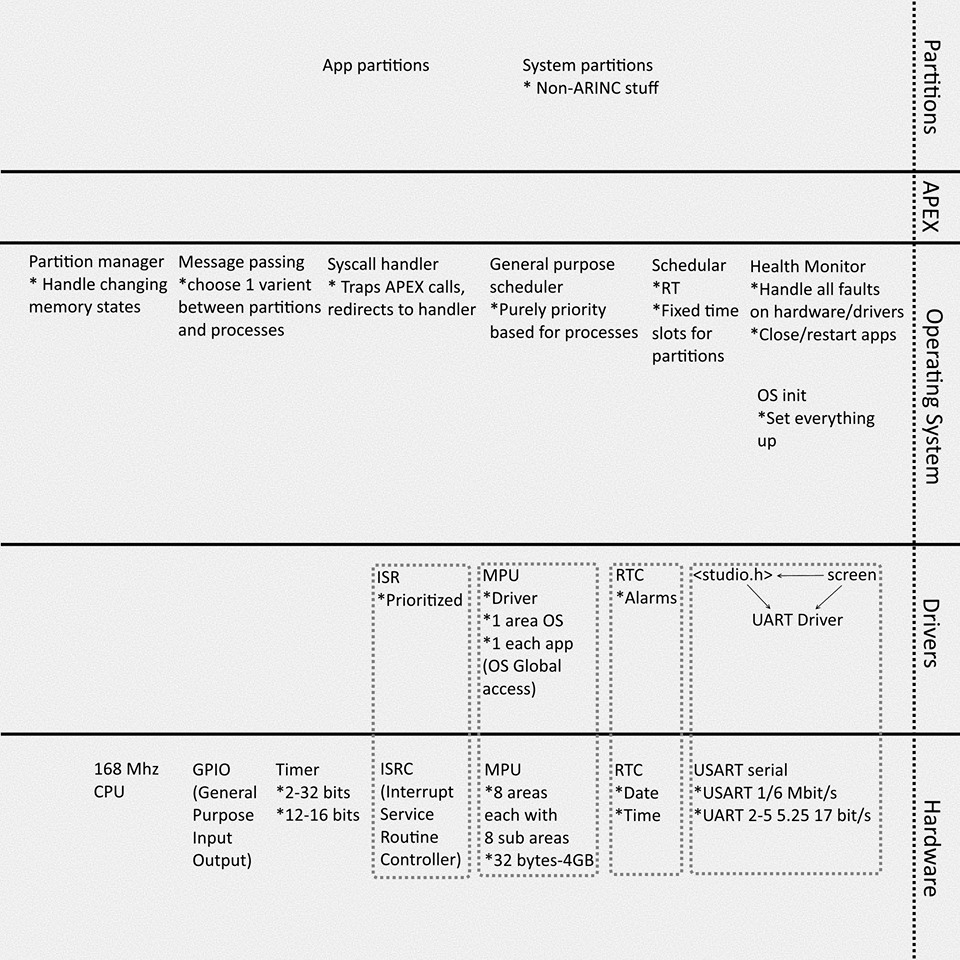
\includegraphics[width=13cm]{first_draft_sys_design_diag.jpeg}

\subsection{Layers}


\subsection{Hardware}

\subsection{Drivers}
\begin{description}[align=left]
	\item [\textbf{UART driver}] The UART is used by the system to communicate with the outside
	world. This can either receive or transmit data to another UART device.
	\item [\textbf{Watchdog timer driver}] The watchdog timer is necessary to ensure recovery
	in case of a hardware fault or program error. If this happens, the program would be restarted
	from a safe state. 
	
\end{description}

\subsection{OS}
\subsubsection{Scheduler}
Here we have some nice text about the scheduler(s).

\paragraph{Context switching} is an absolute necessity in a multitasking operating system.
Context switching works by dumping the CPU registers from one context to memory,
and then switching to another context by restoring the registers from another dump.
Since context switching must manipulate registers directly and individually, it is a feature that must be implemented
on a very low level of abstraction, and it can change significantly from one CPU architecture to another.
The scope of this project is to only implement an operating system for a Cortex M4. Hence context switching needs only
to work on the architecture used by this chip.\\
Context Switching on the Cortex M4 is partially handled by the Nested Vectored Interrupt Controller (NVIC).
When an exception (this includes interrupts) occurs, the NVIC will change context to an exception handler.
Upon changing context from regular code to the exception handler, the NVIC will save the registers R0-R3, R12, LR, PC and PSR
on the stack. These are only some of the registers. Why the decision was made to make the hardware save some of the 
registers instead of letting software handle all, is unknown. \todo{Research harder the reason why the NVIC saves some register.}
When the exception handling routine exits, and control is handed back to the NVIC,
the NVIC will restore these registers again.\\
If the operating system wishes to switch context, it must save the remaining registers, R4-R11, and the stack pointer to memory 
pick a new context to restore, reload the registers R4-R11 and the stack pointer of the new context from memory,
and hand back control to the NVIC. The NVIC will then reload the remaining registers from the stack of the new context.\\\\
As added complexity, the Cortex M4 utilises two different stack pointers, the Master Stack Pointer (MSP) and the Process Stack Pointer (PSP).
The MSP is intended for kernel space execution and the PSP is intended for user space execution, but there is no enforcement.
Switching between the two cannot be done in an exception handler, but must instead be done by the NVIC.
The way to communicate which stack pointer to use with the NVIC, is to load the Program Counter register with a certain value (see EXC\_RETURN values). 


\subsubsection{Interpartition communication}

\section{XML}


\section{Memory Management}
ARINC 653 advertizes time and space seperation covered in (ref to sec in analysis).
To accommodate for the feature of seperating partitions in space
this operating system relies on the memory management unit (MPU)
to manage permissions accross sections of memory
ensuring that partitions stay within a dedicated memory space.

\subsection{something about ARINC on memory management}

\subsection{the MPU on a STM32F415}

\subsection{memory strategy}
